% Cours de mathématiques pour la classe de 4e – année scolaire 2025‑2026
% Fichier principal - Structure modulaire

\documentclass[12pt,a4paper]{book}
% ================================
% PACKAGES ET CONFIGURATIONS
% ================================
% Encodage et langue
\usepackage[utf8]{inputenc}
\usepackage[T1]{fontenc}
\usepackage[french]{babel}
% Mise en page
\usepackage[top=2.5cm, bottom=2.5cm, left=2.5cm, right=2.5cm]{geometry}
\usepackage{fancyhdr}
\usepackage{titlesec}
\usepackage{tocloft}
% Mathématiques
\usepackage{amsmath, amssymb, amsfonts}
\usepackage{mathtools}
\usepackage{xfrac}
% Figures et couleurs
\usepackage{tikz}
\usepackage{pgfplots}
\usepackage{xcolor}
\usepackage{graphicx}
\usepackage{float}
% Tableaux et listes
\usepackage{array}
\usepackage{tabularx}
\usepackage{enumitem}
% Boîtes et encadrés
\usepackage{tcolorbox}
\usepackage{mdframed}
% ================================
% DÉFINITION DES COULEURS
% ================================
\definecolor{bleuprincippal}{RGB}{41, 128, 185}
\definecolor{vertaccent}{RGB}{39, 174, 96}
\definecolor{rougeaccent}{RGB}{231, 76, 60}
\definecolor{grisfonce}{RGB}{52, 73, 94}
\definecolor{grisclair}{RGB}{236, 240, 241}
% ================================
% CONFIGURATION DES TITRES
% ================================
% Style des chapitres
\titleformat{\chapter}[display]
  {\normalfont\huge\bfseries\color{bleuprincippal}}
  {\chaptertitlename\ \thechapter}{20pt}{\Huge}
% Style des sections
\titleformat{\section}
  {\normalfont\Large\bfseries\color{bleuprincippal}}
  {\thesection}{1em}{}
% Style des subsections
\titleformat{\subsection}
  {\normalfont\large\bfseries\color{grisfonce}}
  {\thesubsection}{1em}{}
% ================================
% CONFIGURATION DES EN‑TÊTES
% ================================
\pagestyle{fancy}
\fancyhf{}
\fancyhead[LE]{\textcolor{bleuprincippal}{\leftmark}}
\fancyhead[RO]{\textcolor{bleuprincippal}{\rightmark}}
\fancyfoot[C]{\textcolor{grisfonce}{\thepage}}
\renewcommand{\headrulewidth}{1pt}
\renewcommand{\headrule}{\hbox to\headwidth{\color{bleuprincippal}\leaders\hrule height \headrulewidth\hfill}}
% ================================
% BOÎTES PERSONNALISÉES
% ================================
% Définition
\newtcolorbox{definition}[1]{
  colback=bleuprincippal!10,
  colframe=bleuprincippal,
  fonttitle=\bfseries,
  title=Définition : #1,
  sharp corners,
  boxrule=1pt
}
% Propriété
\newtcolorbox{propriete}[1]{
  colback=vertaccent!10,
  colframe=vertaccent,
  fonttitle=\bfseries,
  title=Propriété : #1,
  sharp corners,
  boxrule=1pt
}
% Méthode
\newtcolorbox{methode}[1]{
  colback=rougeaccent!10,
  colframe=rougeaccent,
  fonttitle=\bfseries,
  title=Méthode : #1,
  sharp corners,
  boxrule=1pt
}
% Exemple
\newtcolorbox{exemple}{
  colback=grisclair,
  colframe=grisfonce,
  fonttitle=\bfseries,
  title=Exemple,
  sharp corners,
  boxrule=1pt
}
% Exercice
\newtcolorbox{exercice}[1]{
  colback=white,
  colframe=grisfonce,
  fonttitle=\bfseries,
  title=Exercice #1,
  sharp corners,
  boxrule=1pt
}
% ================================
% INFORMATIONS DU DOCUMENT
% ================================
\title{
  \vspace{-2cm}
  \begin{tikzpicture}[remember picture, overlay]
    \fill[bleuprincippal] (current page.north west) rectangle ([yshift=-3cm]current page.north east);
  \end{tikzpicture}
  \vspace{1cm}
  {\Huge\color{white}\textbf{MATHÉMATIQUES}}\\[0.5cm]
  {\Large\color{white}Classe de 4\textsuperscript{e}}\\[0.3cm]
  {\large\color{white}Programme 2025-2026}
}
\author{
  \textcolor{grisfonce}{\Large M. Abdoullatuf}\\
  \textcolor{grisfonce}{Collège Sainte Jeanne d'Arc}
}
\date{
  \textcolor{grisfonce}{Année scolaire 2025-2026}
}
% ================================
% DÉBUT DU DOCUMENT
% ================================
\begin{document}
% Page de titre
\maketitle
\thispagestyle{empty}
% Table des matières
\tableofcontents
\newpage

% ================================
% INCLUSION DES CHAPITRES
% ================================

% PARTIE I : NOMBRES ET CALCULS
\part{Nombres et Calculs}
% Chapitre 1 : Nombres relatifs (1)
\chapter{Nombres relatifs (1)}

\section{Introduction :}
Les nombres relatifs sont utilisés dans de nombreuses situations de la vie quotidienne : pour mesurer des températures, des altitudes, des soldes bancaires, ou pour se repérer dans le temps. Ils nous permettent de décrire des quantités qui peuvent être positives (au-dessus de zéro) ou négatives (en dessous de zéro).

\section{Rappels: Définition et Représentation}
\begin{definition}{Nombre relatif}
Un nombre relatif est un nombre qui peut être positif, négatif ou nul.
\end{definition}

\subsection{La droite graduée}
Un nombre relatif est repéré par son signe (+ ou -) et sa distance à zéro.\newline
Sur une droite graduée, le point de référence est l'origine (0).
\begin{itemize}[label=\textbullet]
\item Les nombres positifs sont à droite de 0.
\item Les nombres négatifs sont à gauche de 0.
\end{itemize}

\subsection{Distance à zéro}
La distance à zéro d'un nombre relatif est la distance qui le sépare de 0 sur la droite graduée. C'est un nombre \textbf{toujours positif}.
\begin{exemple}
La distance à zéro de +6 est 6. La distance à zéro de -4,5 est 4,5.
\end{exemple}

\subsection{Nombres opposés}
Deux nombres sont \textbf{opposés} s'ils ont la \textbf{même distance à zéro} mais des \textbf{signes différents}. Leur somme est toujours égale à 0.
\begin{exemple}
L'opposé de +7 est -7. L'opposé de -2,3 est +2,3.
\end{exemple}

\begin{propriete}{Additionner deux nombres de MÊME SIGNE}
Pour additionner deux nombres relatifs de même signe:
\begin{itemize}[label=\textbullet]
\item On \textbf{garde le signe commun}.
\item On \textbf{additionne} leurs distances à zéro.
\end{itemize}
\end{propriete}
\begin{exemple}
$(+5) + (+9) = +14 \ (\text{Le signe commun est +, et}\ 5 + 9 = 14)$\\
$(-7) + (-3) = -10 \ (\text{Le signe commun est -, et}\ 7 + 3 = 10)$\\
(-1,5) + (-4) = -5,5
\end{exemple}

\section{Multiplication et division}
\begin{methode}{Règle des signes}
\begin{itemize}
\item Le produit de deux nombres de même signe est positif
\item Le produit de deux nombres de signes contraires est négatif
\end{itemize}
\end{methode} 
% Chapitre 2 : Théorème de Pythagore et sa réciproque
% Version améliorée conforme à la réforme du collège 2025
\chapter{Théorème de Pythagore et sa réciproque}

\section{Introduction}
Le théorème de Pythagore est l'un des théorèmes les plus célèbres et les plus utiles de la géométrie. Il porte le nom de Pythagore, mathématicien et philosophe grec du VI\textsuperscript{e} siècle avant J.-C., bien que cette relation ait été découverte par plusieurs civilisations antérieures (Babyloniens, Égyptiens, Chinois).

Ce théorème établit une relation fondamentale entre les côtés d'un triangle rectangle et trouve de nombreuses applications dans la vie courante : architecture, navigation, cartographie, sport, etc.

\textbf{Problématique du chapitre :} Comment calculer des longueurs dans un triangle rectangle ? Comment déterminer si un triangle est rectangle ?

\section{Activité d'approche : découverte par manipulation}

\textbf{Objectif :} Découvrir la relation entre les aires des carrés construits sur les côtés d'un triangle rectangle.

\textbf{Matériel :} Papier quadrillé, ciseaux, règle graduée

\textbf{Consigne :}
\begin{enumerate}
    \item Construire plusieurs triangles rectangles sur papier quadrillé
    \item Construire un carré sur chacun des trois côtés
    \item Compter le nombre de carreaux de chaque carré
    \item Chercher une relation entre ces trois nombres
\end{enumerate}

\textbf{Constat :} Pour tout triangle rectangle, l'aire du carré construit sur l'hypoténuse est égale à la somme des aires des carrés construits sur les deux autres côtés.

\section{Définitions et vocabulaire}

\begin{definition}{Triangle rectangle}
Triangle ayant un angle droit (90°).
\end{definition}

\begin{definition}{Hypoténuse}
Côté opposé à l'angle droit dans un triangle rectangle. C'est le plus long côté du triangle.
\end{definition}

\begin{definition}{Côtés de l'angle droit}
Les deux côtés qui forment l'angle droit.
\end{definition}

\section{Le théorème de Pythagore}

\subsection{Énoncé du théorème}

\begin{propriete}{Théorème de Pythagore}
Dans un triangle rectangle, le carré de la longueur de l'hypoténuse est égal à la somme des carrés des longueurs des deux autres côtés.
\end{propriete}

\textbf{Formulation mathématique :}\\
Si $ABC$ est un triangle rectangle en $A$, alors : $BC^2 = AB^2 + AC^2$

\begin{center}
\begin{tikzpicture}[scale=1.2]
    % Triangle rectangle
    \coordinate (A) at (0,0);
    \coordinate (B) at (3,0);
    \coordinate (C) at (0,2);
    
    % Tracé du triangle
    \draw[thick] (A) -- (B) -- (C) -- cycle;
    
    % Angle droit
    \draw (0.3,0) -- (0.3,0.3) -- (0,0.3);
    
    % Étiquettes
    \node[below left] at (A) {$A$};
    \node[below right] at (B) {$B$};
    \node[above left] at (C) {$C$};
    
    % Côtés
    \node[below] at (1.5,0) {$c$};
    \node[left] at (0,1) {$b$};
    \node[above right] at (1.5,1) {$a$ (hypoténuse)};
\end{tikzpicture}
\end{center}

\subsection{Démonstration par la méthode des aires}

Considérons un carré de côté $(a + b)$ contenant quatre triangles rectangles identiques de côtés $a$, $b$ et d'hypoténuse $c$.

\begin{figure}[H]
\centering
\begin{minipage}{0.45\textwidth}
    \centering
    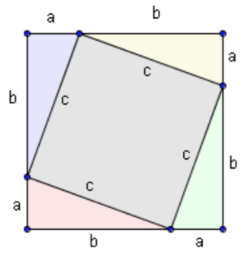
\includegraphics[width=0.8\textwidth]{chapitres/figures/chapitre_02_pythagore/fig_demo_pythagore_config_1.png}
    \caption{Configuration 1}
    \label{fig:config1}
\end{minipage}
\hfill
\begin{minipage}{0.45\textwidth}
    \centering
    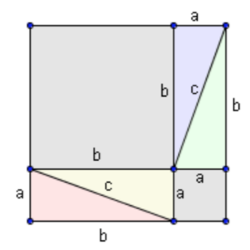
\includegraphics[width=0.8\textwidth]{chapitres/figures/chapitre_02_pythagore/fig_demo_pythagore_config_2.png}
    \caption{Configuration 2}
    \label{fig:config2}
\end{minipage}
\end{figure}

\textbf{Configuration 1 :} Aires = $(a+b)^2 = 4 \times \frac{ab}{2} + c^2 = 2ab + c^2$

\textbf{Configuration 2 :} Aires = $(a+b)^2 = 4 \times \frac{ab}{2} + a^2 + b^2 = 2ab + a^2 + b^2$

Comme l'aire est la même dans les deux configurations :
\[c^2 = a^2 + b^2\]

Ce qui démontre le théorème de Pythagore.

\section{Applications du théorème de Pythagore}

\subsection{Calculer la longueur de l'hypoténuse}

\begin{methode}{Calculer la longueur de l'hypoténuse}
Pour calculer la longueur de l'hypoténuse d'un triangle rectangle :
\begin{enumerate}
    \item Identifier le triangle rectangle et ses côtés
    \item Repérer l'hypoténuse (côté opposé à l'angle droit)
    \item Appliquer la formule : hypoténuse$^2$ = côté$_1^2$ + côté$_2^2$
    \item Calculer la racine carrée du résultat
\end{enumerate}
\end{methode}

\begin{exemple}
Un triangle $ABC$ est rectangle en $A$. $AB = 6$ cm et $AC = 8$ cm.\\
Calculer $BC$.

\textbf{Solution :}
\begin{itemize}
    \item Le triangle est rectangle en $A$, donc $BC$ est l'hypoténuse
    \item D'après le théorème de Pythagore : $BC^2 = AB^2 + AC^2$
    \item $BC^2 = 6^2 + 8^2 = 36 + 64 = 100$
    \item $BC = \sqrt{100} = 10$ cm
\end{itemize}
\end{exemple}

\subsection{Calculer la longueur d'un côté de l'angle droit}

\begin{methode}{Calculer la longueur d'un côté de l'angle droit}
Pour calculer la longueur d'un côté de l'angle droit :
\begin{enumerate}
    \item Identifier la longueur de l'hypoténuse et celle de l'autre côté de l'angle droit
    \item Appliquer la formule : hypoténuse$^2$ = côté$_1^2$ + côté$_2^2$
    \item Isoler le côté inconnu : côté$^2$ = hypoténuse$^2$ - autre côté$^2$
    \item Calculer la racine carrée du résultat
\end{enumerate}
\end{methode}

\begin{exemple}
Un triangle $DEF$ est rectangle en $D$. $DE = 5$ cm et $EF = 13$ cm.\\
Calculer $DF$.

\textbf{Solution :}
\begin{itemize}
    \item Le triangle est rectangle en $D$, donc $EF$ est l'hypoténuse
    \item D'après le théorème de Pythagore : $EF^2 = DE^2 + DF^2$
    \item $13^2 = 5^2 + DF^2$
    \item $169 = 25 + DF^2$
    \item $DF^2 = 169 - 25 = 144$
    \item $DF = \sqrt{144} = 12$ cm
\end{itemize}
\end{exemple}

\section{La réciproque du théorème de Pythagore}

\subsection{Énoncé de la réciproque}

\begin{propriete}{Réciproque du théorème de Pythagore}
Si, dans un triangle, le carré de la longueur du plus grand côté est égal à la somme des carrés des longueurs des deux autres côtés, alors ce triangle est rectangle.
\end{propriete}

\subsection{Utilisation de la réciproque}

\textbf{Objectif :} Déterminer si un triangle est rectangle en connaissant les longueurs de ses trois côtés.

\begin{methode}{Démontrer qu'un triangle est rectangle}
Pour démontrer qu'un triangle est rectangle :
\begin{enumerate}
    \item Identifier le plus grand côté du triangle
    \item Calculer le carré de sa longueur
    \item Calculer la somme des carrés des deux autres côtés
    \item Comparer les résultats :
    \begin{itemize}
        \item Si égalité : le triangle est rectangle
        \item Si inégalité : le triangle n'est pas rectangle
    \end{itemize}
\end{enumerate}
\end{methode}

\begin{exemple}
Un triangle a pour côtés 9 cm, 12 cm et 15 cm. Est-il rectangle ?

\textbf{Solution :}
\begin{itemize}
    \item Le plus grand côté mesure 15 cm
    \item $15^2 = 225$
    \item $9^2 + 12^2 = 81 + 144 = 225$
    \item Puisque $15^2 = 9^2 + 12^2$, le triangle est rectangle
    \item L'angle droit est opposé au côté de 15 cm
\end{itemize}
\end{exemple}

\begin{exemple}
Un triangle a pour côtés 7 cm, 8 cm et 10 cm. Est-il rectangle ?

\textbf{Solution :}
\begin{itemize}
    \item Le plus grand côté mesure 10 cm
    \item $10^2 = 100$
    \item $7^2 + 8^2 = 49 + 64 = 113$
    \item Puisque $100 \neq 113$, le triangle n'est pas rectangle
\end{itemize}
\end{exemple}

\section{Applications et résolution de problèmes}

\subsection{Problèmes de la vie courante}

\begin{exercice}{1 - L'échelle}
Une échelle de 4 m est appuyée contre un mur. Son pied est à 1,5 m du mur. À quelle hauteur le sommet de l'échelle touche-t-il le mur ?

\textbf{Solution :}
\begin{itemize}
    \item Triangle rectangle : mur, sol, échelle
    \item Hypoténuse : échelle = 4 m
    \item Un côté : distance au mur = 1,5 m
    \item Autre côté : hauteur = ?
\end{itemize}

$h^2 + 1,5^2 = 4^2$\\
$h^2 + 2,25 = 16$\\
$h^2 = 13,75$\\
$h = \sqrt{13,75} \approx 3,7$ m
\end{exercice}

\begin{exercice}{2 - Vérification d'équerrage}
Un maçon vérifie qu'un angle est droit en mesurant les côtés d'un triangle formé par deux murs et une diagonale. Il mesure : 3 m, 4 m et 5 m. L'angle est-il droit ?

\textbf{Solution :}
\begin{itemize}
    \item Plus grand côté : 5 m
    \item $5^2 = 25$
    \item $3^2 + 4^2 = 9 + 16 = 25$
    \item Égalité vérifiée $\Rightarrow$ l'angle est droit
\end{itemize}
\end{exercice}

\subsection{Utilisation de la calculatrice}

\textbf{Compétence :} Utiliser la touche $\sqrt{}$ (racine carrée) de la calculatrice.

\textbf{Exemple :} Calculer $\sqrt{75}$
\begin{itemize}
    \item $\sqrt{75} = \sqrt{25 \times 3} = \sqrt{25} \times \sqrt{3} = 5\sqrt{3} \approx 8,66$
\end{itemize}

\subsection{Calculs exacts et valeurs approchées}

\textbf{Calcul exact :} $\sqrt{50} = \sqrt{25 \times 2} = 5\sqrt{2}$ cm\\
\textbf{Valeur approchée :} $\sqrt{50} \approx 7,07$ cm (arrondi au centième)

\section{Théorème de Pythagore dans l'espace}

\subsection{Distance dans un pavé droit}

\textbf{Problème :} Calculer la longueur de la diagonale d'un pavé droit.

Pour un pavé droit de dimensions $a$, $b$ et $c$, la diagonale $d$ vérifie :
\[d^2 = a^2 + b^2 + c^2\]

\begin{exemple}
Pavé droit de dimensions 6 cm × 8 cm × 5 cm\\
$d^2 = 6^2 + 8^2 + 5^2 = 36 + 64 + 25 = 125$\\
$d = \sqrt{125} = 5\sqrt{5} \approx 11,18$ cm
\end{exemple}

\section{Compétences travaillées et automatismes}

\subsection{Compétences du socle commun}

\begin{itemize}
    \item \textbf{Chercher :} Identifier un triangle rectangle, choisir la bonne méthode
    \item \textbf{Modéliser :} Traduire un problème concret en calcul mathématique
    \item \textbf{Représenter :} Faire un schéma, coder une figure
    \item \textbf{Raisonner :} Justifier qu'un triangle est ou n'est pas rectangle
    \item \textbf{Calculer :} Effectuer des calculs avec des radicaux
    \item \textbf{Communiquer :} Rédiger une solution complète
\end{itemize}

\subsection{Automatismes à acquérir}

\begin{itemize}
    \item Reconnaître un triangle rectangle
    \item Identifier l'hypoténuse
    \item Appliquer le théorème direct ou sa réciproque
    \item Utiliser la calculatrice pour les racines carrées
    \item Connaître les "triplets pythagoriciens" usuels : (3;4;5), (5;12;13), (8;15;17)
\end{itemize}

\section{Exercices d'entraînement}

\subsection{Exercices de base}

\begin{exercice}{3}
Calculs directs :
\begin{enumerate}[label=\alph*)]
    \item Triangle rectangle : côtés 3 cm et 4 cm. Calculer l'hypoténuse.
    \item Triangle rectangle : hypoténuse 10 cm, un côté 6 cm. Calculer l'autre côté.
\end{enumerate}
\end{exercice}

\begin{exercice}{4}
Réciproque : Les triangles suivants sont-ils rectangles ?
\begin{enumerate}[label=\alph*)]
    \item Côtés : 7 cm, 24 cm, 25 cm
    \item Côtés : 6 cm, 7 cm, 8 cm
\end{enumerate}
\end{exercice}

\subsection{Exercices d'approfondissement}

\begin{exercice}{5}
\textbf{Problème du terrain}\\
Un terrain rectangulaire mesure 40 m sur 30 m. Calculer la longueur de sa diagonale.
\end{exercice}

\begin{exercice}{6}
\textbf{Navigation}\\
Un bateau part d'un port et navigue 12 km vers l'est puis 5 km vers le nord. À quelle distance se trouve-t-il du port ?
\end{exercice}

\begin{exercice}{7}
\textbf{Architecture}\\
Pour vérifier qu'un mur est perpendiculaire au sol, un architecte place un point A sur le mur à 3 m du sol, un point B au pied du mur, et un point C sur le sol à 4 m de B. Si AC = 5 m, le mur est-il perpendiculaire au sol ?
\end{exercice}

\section{Activité avec les TICE}

\subsection{Utilisation d'un logiciel de géométrie dynamique}

\textbf{Objectif :} Vérifier le théorème de Pythagore avec GeoGebra ou similaire

\textbf{Consignes :}
\begin{enumerate}
    \item Construire un triangle rectangle ABC
    \item Construire les carrés sur chaque côté
    \item Afficher les aires des trois carrés
    \item Modifier la forme du triangle et observer
    \item Conjecture sur la relation entre ces aires
\end{enumerate}

\section{Liens avec d'autres notions mathématiques}

\subsection{Distance entre deux points dans un repère}

Le théorème de Pythagore permet de calculer la distance entre deux points dans un repère orthonormé.

Si $A(x_A, y_A)$ et $B(x_B, y_B)$ sont deux points dans un repère orthonormé, alors la distance $AB$ est donnée par :
\[AB = \sqrt{(x_B - x_A)^2 + (y_B - y_A)^2}\]

\begin{exemple}
Calculons la distance entre les points $A(2, 3)$ et $B(6, 7)$ dans un repère orthonormé.

En appliquant le théorème de Pythagore :
\[AB^2 = (6-2)^2 + (7-3)^2 = 4^2 + 4^2 = 16 + 16 = 32\]
\[AB = \sqrt{32} = \sqrt{16 \times 2} = 4\sqrt{2}\]

La distance entre $A$ et $B$ est $4\sqrt{2}$ unités.
\end{exemple}

\subsection{Équations et théorème de Pythagore}

Le théorème de Pythagore conduit souvent à des équations qu'il faut résoudre pour trouver des longueurs.

\begin{exemple}
Dans un triangle rectangle $ABC$ rectangle en $A$, on sait que $AB = x$ cm, $AC = (x+3)$ cm et $BC = 17$ cm. Déterminons la valeur de $x$.

D'après le théorème de Pythagore :
\[BC^2 = AB^2 + AC^2\]
\[17^2 = x^2 + (x+3)^2\]
\[289 = x^2 + x^2 + 6x + 9\]
\[289 = 2x^2 + 6x + 9\]
\[2x^2 + 6x - 280 = 0\]
\[x^2 + 3x - 140 = 0\]

En factorisant : $(x - 10)(x + 14) = 0$

Les solutions sont $x = 10$ et $x = -14$.

Comme une longueur ne peut pas être négative, nous avons $x = 10$ cm.

Donc $AB = 10$ cm et $AC = 13$ cm.
\end{exemple}

\section{Pour aller plus loin}

\subsection{Histoire des mathématiques}
\begin{itemize}
    \item Les tablettes babyloniennes (Plimpton 322)
    \item La démonstration par le président Garfield
    \item Les différentes démonstrations du théorème (plus de 300 connues)
\end{itemize}

\subsection{Généralisation}
\begin{itemize}
    \item Théorème de Pythagore généralisé (loi des cosinus)
    \item Théorème de Pythagore dans l'espace à n dimensions
\end{itemize}

\subsection{Applications modernes}
\begin{itemize}
    \item GPS et géolocalisation
    \item Graphisme 3D et jeux vidéo
    \item Architecture et ingénierie
\end{itemize}

\section{Synthèse du chapitre}

\textbf{Ce qu'il faut retenir :}

\begin{enumerate}
    \item \textbf{Théorème de Pythagore :} Dans un triangle rectangle, hypoténuse$^2$ = côté$_1^2$ + côté$_2^2$
    \item \textbf{Réciproque :} Si dans un triangle, le carré du plus grand côté égale la somme des carrés des deux autres, alors le triangle est rectangle
    \item \textbf{Applications :} Calcul de longueurs, vérification d'angles droits, résolution de problèmes concrets
    \item \textbf{Méthodes :} Identification du triangle rectangle, application des formules, utilisation de la calculatrice
\end{enumerate}

\textbf{Liens avec d'autres chapitres :}
\begin{itemize}
    \item Racines carrées (chapitre précédent)
    \item Trigonométrie (chapitre à venir)
    \item Géométrie dans l'espace
    \item Fonctions (distance entre deux points dans un repère)
\end{itemize} 
% Chapitre 3 : Puissances
\chapter{Puissances}

\section{Puissances d'exposant positif}
\begin{definition}{Puissance}
Soit $a$ un nombre et $n$ un entier positif non nul. On définit $a^n = \underbrace{a \times a \times \ldots \times a}_{n \text{ facteurs}}$
\end{definition}

\begin{exemple}
$2^3 = 2 \times 2 \times 2 = 8$\\
$5^2 = 5 \times 5 = 25$
\end{exemple}

\section{Puissances de 10}
\begin{propriete}{Notation scientifique}
Tout nombre décimal non nul peut s'écrire sous la forme $a \times 10^n$ où $1 \leq |a| < 10$ et $n$ est un entier relatif.
\end{propriete}

\begin{exemple}
$1234 = 1,234 \times 10^3$\\
$0,00056 = 5,6 \times 10^{-4}$
\end{exemple}

\section{Propriétés des puissances}
\begin{propriete}{Règles de calcul}
Pour tous nombres $a$ et $b$ non nuls et tous entiers $m$ et $n$ :
\begin{itemize}
    \item $a^m \times a^n = a^{m+n}$
    \item $\frac{a^m}{a^n} = a^{m-n}$
    \item $(a^m)^n = a^{m \times n}$
    \item $(a \times b)^n = a^n \times b^n$
    \item $\left(\frac{a}{b}\right)^n = \frac{a^n}{b^n}$
\end{itemize}
\end{propriete}

\section{Puissances d'exposant négatif}
\begin{definition}{Puissance d'exposant négatif}
Pour tout nombre $a$ non nul et tout entier positif $n$ :
$a^{-n} = \frac{1}{a^n}$
\end{definition}

\begin{exemple}
$2^{-3} = \frac{1}{2^3} = \frac{1}{8}$\\
$10^{-2} = \frac{1}{10^2} = \frac{1}{100} = 0,01$
\end{exemple} 
% Chapitre 4 : Racines carrées
\chapter{Racines carrées}

\section{Définition et propriétés}
\begin{definition}{Racine carrée}
La racine carrée d'un nombre positif $a$ est le nombre positif dont le carré est égal à $a$. On la note $\sqrt{a}$.
\end{definition}

\begin{exemple}
$\sqrt{16} = 4$ car $4^2 = 16$\\
$\sqrt{25} = 5$ car $5^2 = 25$
\end{exemple}

\section{Propriétés des racines carrées}
\begin{propriete}{Propriétés fondamentales}
Pour tous nombres positifs $a$ et $b$ :
\begin{itemize}
    \item $\sqrt{a \times b} = \sqrt{a} \times \sqrt{b}$
    \item $\sqrt{\frac{a}{b}} = \frac{\sqrt{a}}{\sqrt{b}}$ (si $b \neq 0$)
    \item $\sqrt{a^2} = |a|$
\end{itemize}
\end{propriete}

\section{Simplification des racines carrées}
\begin{methode}{Simplifier une racine carrée}
Pour simplifier $\sqrt{a}$ :
\begin{enumerate}
    \item Décomposer $a$ en produit de facteurs premiers
    \item Regrouper les facteurs par paires
    \item Extraire les racines carrées des carrés parfaits
\end{enumerate}
\end{methode}

\begin{exemple}
Simplifions $\sqrt{72}$ :
\begin{itemize}
    \item $72 = 2^3 \times 3^2 = 2^2 \times 2 \times 3^2$
    \item $\sqrt{72} = \sqrt{2^2 \times 2 \times 3^2} = \sqrt{2^2} \times \sqrt{3^2} \times \sqrt{2}$
    \item $\sqrt{72} = 2 \times 3 \times \sqrt{2} = 6\sqrt{2}$
\end{itemize}
\end{exemple}

\section{Calculs avec les racines carrées}
\begin{propriete}{Addition et soustraction}
On ne peut additionner ou soustraire que des racines carrées de même radicande :
$\sqrt{a} + \sqrt{a} = 2\sqrt{a}$
\end{propriete}

\begin{exemple}
$\sqrt{3} + \sqrt{3} = 2\sqrt{3}$\\
$\sqrt{5} + \sqrt{3}$ ne peut pas être simplifié
\end{exemple} 
% Chapitre 5 : Nombres premiers et divisibilité
\chapter{Nombres premiers et divisibilité}

\section{Nombres premiers}
\begin{definition}{Nombre premier}
Un nombre premier est un entier naturel qui admet exactement deux diviseurs : 1 et lui-même.
\end{definition}

\begin{exemple}
Les nombres premiers inférieurs à 20 sont : 2, 3, 5, 7, 11, 13, 17, 19.
\end{exemple}

\section{Décomposition en facteurs premiers}
\begin{methode}{Décomposition}
Pour décomposer un nombre en produit de facteurs premiers, on divise successivement par les nombres premiers dans l'ordre croissant.
\end{methode}

\begin{exemple}
Décomposons 84 en facteurs premiers :
\begin{itemize}
    \item $84 \div 2 = 42$
    \item $42 \div 2 = 21$
    \item $21 \div 3 = 7$
    \item $7 \div 7 = 1$
\end{itemize}
Donc $84 = 2^2 \times 3 \times 7$
\end{exemple}

\section{Divisibilité}
\begin{definition}{Diviseur}
Un nombre $a$ est diviseur d'un nombre $b$ s'il existe un entier $k$ tel que $b = a \times k$.
\end{definition}

\begin{propriete}{Critères de divisibilité}
\begin{itemize}
    \item Un nombre est divisible par 2 s'il se termine par 0, 2, 4, 6 ou 8
    \item Un nombre est divisible par 3 si la somme de ses chiffres est divisible par 3
    \item Un nombre est divisible par 5 s'il se termine par 0 ou 5
    \item Un nombre est divisible par 9 si la somme de ses chiffres est divisible par 9
\end{itemize}
\end{propriete} 

% PARTIE II : ORGANISATION ET GESTION DE DONNÉES
\part{Organisation et Gestion de Données}
% Chapitre 6 : Proportionnalité
\chapter{Proportionnalité}

\section{Reconnaissance d'une situation de proportionnalité}
\begin{definition}{Proportionnalité}
Deux grandeurs sont proportionnelles si l'on peut passer de l'une à l'autre en multipliant par un nombre constant appelé coefficient de proportionnalité.
\end{definition}

\begin{exemple}
Le prix payé est proportionnel au nombre d'objets achetés. Si 3 objets coûtent 15€, alors 6 objets coûtent 30€.
\end{exemple}

\section{Pourcentages et échelles}
\begin{definition}{Pourcentage}
Un pourcentage est une fraction dont le dénominateur est 100.
\end{definition}

\begin{methode}{Calculer un pourcentage}
Pour calculer $p\%$ d'un nombre $a$ :
$\frac{p}{100} \times a$
\end{methode}

\begin{exemple}
Calculer 15\% de 200€ :
$\frac{15}{100} \times 200 = 0,15 \times 200 = 30$€
\end{exemple}

\section{Échelle}
\begin{definition}{Échelle}
L'échelle d'une carte ou d'un plan est le rapport entre une distance sur le document et la distance réelle correspondante.
\end{definition}

\begin{exemple}
Sur une carte à l'échelle 1:50000, 1 cm sur la carte représente 50000 cm = 500 m en réalité.
\end{exemple} 
% Chapitre 7 : Statistiques
\chapter{Statistiques}

\section{Médiane}
\begin{definition}{Médiane}
La médiane d'une série statistique est la valeur qui partage cette série ordonnée en deux parties de même effectif.
\end{definition}

\begin{exemple}
Pour la série : 2, 4, 7, 8, 9, 12, 15\\
La médiane est 8 (4 valeurs avant, 4 valeurs après).
\end{exemple}

\section{Diagrammes circulaires}
\begin{definition}{Diagramme circulaire}
Un diagramme circulaire (ou camembert) représente les effectifs ou les fréquences d'une série statistique par des secteurs angulaires.
\end{definition}

\begin{methode}{Construire un diagramme circulaire}
\begin{enumerate}
    \item Calculer les angles correspondant à chaque effectif
    \item Tracer les secteurs avec les angles calculés
    \item Ajouter les légendes
\end{enumerate}
\end{methode}

\section{Caractéristiques de position}
\begin{definition}{Moyenne}
La moyenne d'une série statistique est la somme de toutes les valeurs divisée par l'effectif total.
\end{definition}

\begin{exemple}
Pour la série : 12, 15, 18, 20, 25\\
La moyenne est : $\frac{12 + 15 + 18 + 20 + 25}{5} = \frac{90}{5} = 18$
\end{exemple} 
% Chapitre 8 : Probabilités
\chapter{Probabilités}

\section{Vocabulaire des probabilités}
\begin{definition}{Expérience aléatoire}
Une expérience aléatoire est une expérience dont on ne peut pas prévoir le résultat à l'avance.
\end{definition}

\begin{definition}{Événement}
Un événement est un ensemble de résultats possibles d'une expérience aléatoire.
\end{definition}

\begin{exemple}
Lancer un dé est une expérience aléatoire.\\
"Obtenir un nombre pair" est un événement.
\end{exemple}

\section{Calcul de probabilités}
\begin{propriete}{Probabilité d'un événement}
La probabilité d'un événement est un nombre compris entre 0 et 1.
\end{propriete}

\begin{definition}{Probabilité}
La probabilité d'un événement $A$ est :
$P(A) = \frac{\text{nombre de cas favorables}}{\text{nombre de cas possibles}}$
\end{definition}

\begin{exemple}
Dans un jeu de 32 cartes, la probabilité de tirer un as est :
$P(\text{as}) = \frac{4}{32} = \frac{1}{8} = 0,125$
\end{exemple}

\section{Événements particuliers}
\begin{definition}{Événement certain}
Un événement certain a une probabilité égale à 1.
\end{definition}

\begin{definition}{Événement impossible}
Un événement impossible a une probabilité égale à 0.
\end{definition}

\begin{exemple}
Dans un jeu de 32 cartes :
\begin{itemize}
    \item "Tirer une carte" est un événement certain ($P = 1$)
    \item "Tirer un 10 de trèfle" est un événement impossible ($P = 0$)
\end{itemize}
\end{exemple} 

% PARTIE III : CALCUL LITTÉRAL ET ÉQUATIONS
\part{Calcul Littéral et Équations}
% Chapitre 9 : Calcul littéral
\chapter{Calcul littéral}

\section{Expressions littérales}
\begin{definition}{Expression littérale}
Une expression littérale est une expression mathématique dans laquelle un ou plusieurs nombres sont remplacés par des lettres.
\end{definition}

\begin{exemple}
$2x + 3$, $3a^2 - 2b + 1$, $5(x + 2)$ sont des expressions littérales.
\end{exemple}

\section{Développement et factorisation}
\begin{propriete}{Distributivité}
$k(a + b) = ka + kb$ et $k(a - b) = ka - kb$
\end{propriete}

\begin{exemple}
$3(x + 2) = 3x + 6$\\
$2(a - 5) = 2a - 10$
\end{exemple}

\section{Double distributivité}
\begin{propriete}{Double distributivité}
$(a + b)(c + d) = ac + ad + bc + bd$
\end{propriete}

\begin{exemple}
$(x + 2)(x + 3) = x^2 + 3x + 2x + 6 = x^2 + 5x + 6$
\end{exemple}

\section{Identités remarquables}
\begin{propriete}{Identités remarquables}
\begin{itemize}
    \item $(a + b)^2 = a^2 + 2ab + b^2$
    \item $(a - b)^2 = a^2 - 2ab + b^2$
    \item $(a + b)(a - b) = a^2 - b^2$
\end{itemize}
\end{propriete}

\begin{exemple}
$(x + 4)^2 = x^2 + 8x + 16$\\
$(2x - 3)^2 = 4x^2 - 12x + 9$\\
$(x + 2)(x - 2) = x^2 - 4$
\end{exemple} 
% Chapitre 10 : Équations
\chapter{Équations}

\section{Résolution d'équations du premier degré}
\begin{definition}{Équation}
Une équation est une égalité dans laquelle intervient un nombre inconnu, généralement représenté par une lettre.
\end{definition}

\begin{methode}{Résolution d'une équation}
Pour résoudre une équation, on peut ajouter ou soustraire un même nombre aux deux membres, ou multiplier ou diviser les deux membres par un même nombre non nul.
\end{methode}

\begin{exemple}
Résolvons l'équation $2x + 3 = 11$ :
\begin{itemize}
    \item $2x + 3 = 11$
    \item $2x + 3 - 3 = 11 - 3$ (on soustrait 3 aux deux membres)
    \item $2x = 8$
    \item $\frac{2x}{2} = \frac{8}{2}$ (on divise par 2 les deux membres)
    \item $x = 4$
\end{itemize}
La solution est $x = 4$.
\end{exemple}

\section{Équations avec fractions}
\begin{methode}{Résoudre une équation avec fractions}
\begin{enumerate}
    \item Réduire au même dénominateur
    \item Multiplier les deux membres par ce dénominateur
    \item Résoudre l'équation obtenue
\end{enumerate}
\end{methode}

\begin{exemple}
Résolvons $\frac{x}{2} + \frac{x}{3} = 5$ :
\begin{itemize}
    \item $\frac{3x}{6} + \frac{2x}{6} = 5$
    \item $\frac{5x}{6} = 5$
    \item $5x = 30$
    \item $x = 6$
\end{itemize}
\end{exemple}

\section{Problèmes se ramenant à une équation}
\begin{methode}{Résoudre un problème}
\begin{enumerate}
    \item Choisir l'inconnue
    \item Traduire le problème par une équation
    \item Résoudre l'équation
    \item Vérifier la solution
\end{enumerate}
\end{methode}

\begin{exemple}
Un nombre augmenté de 5 est égal au double de ce nombre diminué de 3. Quel est ce nombre ?

\textbf{Solution :}
\begin{itemize}
    \item Soit $x$ ce nombre
    \item $x + 5 = 2x - 3$
    \item $x + 5 - x = 2x - 3 - x$
    \item $5 = x - 3$
    \item $5 + 3 = x - 3 + 3$
    \item $8 = x$
\end{itemize}
Le nombre cherché est 8.
\end{exemple} 

% PARTIE IV : FONCTIONS
\part{Fonctions}
% Chapitre 11 : Notion de fonction
\chapter{Notion de fonction}

\section{Dépendance entre deux grandeurs}
\begin{definition}{Fonction}
Une fonction est un processus qui, à un nombre, associe un autre nombre.
\end{definition}

\begin{exemple}
La fonction qui à un nombre associe son double : $f(x) = 2x$
\end{exemple}

\section{Représentation graphique}
\begin{definition}{Courbe représentative}
La courbe représentative d'une fonction $f$ est l'ensemble des points de coordonnées $(x; f(x))$.
\end{definition}

\begin{methode}{Tracer une courbe}
\begin{enumerate}
    \item Calculer quelques valeurs de la fonction
    \item Placer les points correspondants
    \item Relier les points par une courbe
\end{enumerate}
\end{methode}

\section{Fonctions linéaires}
\begin{definition}{Fonction linéaire}
Une fonction linéaire est une fonction de la forme $f(x) = ax$ où $a$ est un nombre fixé.
\end{definition}

\begin{propriete}{Représentation graphique}
La courbe représentative d'une fonction linéaire est une droite passant par l'origine.
\end{propriete}

\begin{exemple}
La fonction $f(x) = 3x$ est une fonction linéaire.
\end{exemple} 

% PARTIE V : GÉOMÉTRIE
\part{Géométrie}
% Chapitre 12 : Théorème de Pythagore (Géométrie)
\chapter{Théorème de Pythagore}

\section{Énoncé et démonstration}
\begin{propriete}{Théorème de Pythagore}
Dans un triangle rectangle, le carré de la longueur de l'hypoténuse est égal à la somme des carrés des longueurs des deux autres côtés.
\end{propriete}

\section{Réciproque du théorème de Pythagore}
\begin{propriete}{Réciproque}
Si, dans un triangle, le carré de la longueur du plus grand côté est égal à la somme des carrés des longueurs des deux autres côtés, alors ce triangle est rectangle.
\end{propriete}

\section{Applications géométriques}
\begin{exemple}
Calculer la diagonale d'un carré de côté 5 cm.
\begin{itemize}
    \item $d^2 = 5^2 + 5^2 = 25 + 25 = 50$
    \item $d = \sqrt{50} = 5\sqrt{2}$ cm
\end{itemize}
\end{exemple} 
\input{chapitres/chapitre_13_thalès}
% Chapitre 14 : Trigonométrie
\chapter{Trigonométrie}

\section{Cosinus d'un angle aigu}
\begin{definition}{Cosinus}
Dans un triangle rectangle, le cosinus d'un angle aigu est le rapport de la longueur du côté adjacent à cet angle sur la longueur de l'hypoténuse.
\end{definition}

\begin{exemple}
Dans un triangle rectangle ABC rectangle en A :
$\cos(\widehat{B}) = \frac{AB}{BC}$
\end{exemple}

\section{Sinus et tangente}
\begin{definition}{Sinus}
Le sinus d'un angle aigu est le rapport de la longueur du côté opposé sur la longueur de l'hypoténuse.
\end{definition}

\begin{definition}{Tangente}
La tangente d'un angle aigu est le rapport de la longueur du côté opposé sur la longueur du côté adjacent.
\end{definition}

\section{Utilisation de la calculatrice}
\begin{methode}{Calculer un angle}
Pour calculer un angle connaissant son cosinus :
\begin{enumerate}
    \item Utiliser la touche $\cos^{-1}$ ou $\arccos$
    \item Entrer la valeur du cosinus
    \item Lire l'angle en degrés
\end{enumerate}
\end{methode} 
% Chapitre 15 : Transformations : Translation
\chapter{Transformations : Translation}

\section{Définition et propriétés}
\begin{definition}{Translation}
Une translation est une transformation qui fait glisser tous les points d'une figure dans la même direction, dans le même sens et sur la même distance.
\end{definition}

\begin{exemple}
La translation de vecteur $\vec{AB}$ transforme tout point $M$ en un point $M'$ tel que $\vec{MM'} = \vec{AB}$.
\end{exemple}

\section{Propriétés de conservation}
\begin{propriete}{Propriétés de la translation}
Une translation conserve :
\begin{itemize}
    \item Les longueurs
    \item Les angles
    \item Les aires
    \item Le parallélisme
    \item L'alignement
\end{itemize}
\end{propriete}

\section{Construction de l'image d'une figure}
\begin{methode}{Construire l'image par translation}
\begin{enumerate}
    \item Construire l'image de quelques points caractéristiques
    \item Relier ces points pour former l'image de la figure
\end{enumerate}
\end{methode} 
% Chapitre 16 : Agrandissement et réduction
\chapter{Agrandissement et réduction}

\section{Effet sur les longueurs, aires et volumes}
\begin{propriete}{Agrandissement}
Dans un agrandissement de rapport $k > 1$ :
\begin{itemize}
  \item Les longueurs sont multipliées par $k$
  \item Les aires sont multipliées par $k^2$
  \item Les volumes sont multipliés par $k^3$
\end{itemize}
\end{propriete}

\begin{propriete}{Réduction}
Dans une réduction de rapport $k$ avec $0 < k < 1$ :
\begin{itemize}
  \item Les longueurs sont multipliées par $k$
  \item Les aires sont multipliées par $k^2$
  \item Les volumes sont multipliés par $k^3$
\end{itemize}
\end{propriete}

\section{Applications}
\begin{exemple}
Un cube de côté 2 cm est agrandi avec un rapport 3.
\begin{itemize}
  \item Nouveau côté : $2 \times 3 = 6$ cm
  \item Nouvelle aire : $24 \times 3^2 = 216$ cm$^2$
  \item Nouveau volume : $8 \times 3^3 = 216$ cm$^3$
\end{itemize}
\end{exemple} 

% PARTIE VI : GRANDEURS ET MESURES
\part{Grandeurs et Mesures}
% Chapitre 17 : Aires et volumes
\chapter{Aires et volumes}

\section{Volume de la pyramide et du cône}
\begin{propriete}{Volume d'une pyramide}
$V = \frac{1}{3} \times \text{Aire de la base} \times \text{hauteur}$
\end{propriete}

\begin{propriete}{Volume d'un cône}
$V = \frac{1}{3} \times \pi \times r^2 \times h$
\end{propriete}

\section{Conversions d'unités composées}
\begin{methode}{Convertir des unités}
\begin{enumerate}
    \item Identifier les unités à convertir
    \item Utiliser les relations entre unités
    \item Effectuer les calculs
\end{enumerate}
\end{methode}

\begin{exemple}
Convertir 2,5 m$^3$ en dm$^3$ :
$2,5$ m$^3 = 2,5 \times 1000 = 2500$ dm$^3$
\end{exemple} 

% PARTIE VII : ALGORITHMIQUE ET PROGRAMMATION
\part{Algorithmique et Programmation}
% Chapitre 18 : Algorithmique
\chapter{Algorithmique}

\section{Instructions conditionnelles}
\begin{definition}{Instruction conditionnelle}
Une instruction conditionnelle permet d'exécuter des actions différentes selon qu'une condition est vraie ou fausse.
\end{definition}

\begin{exemple}
Si $x > 0$ alors afficher "positif" sinon afficher "négatif ou nul"
\end{exemple}

\section{Boucles}
\begin{definition}{Boucle}
Une boucle permet de répéter un ensemble d'instructions un nombre déterminé de fois.
\end{definition}

\begin{exemple}
Pour $i$ de 1 à 5 :
\begin{itemize}
    \item Afficher $i$
    \item Fin pour
\end{itemize}
\end{exemple}

\section{Variables}
\begin{definition}{Variable}
Une variable est un emplacement mémoire qui peut contenir une valeur qui peut changer.
\end{definition}

\begin{exemple}
$x \leftarrow 5$ (affectation)\\
$y \leftarrow x + 3$ (calcul)
\end{exemple} 
% Chapitre 19 : Programmation
\chapter{Programmation}

\section{Variables et calculs}
\begin{definition}{Variable en programmation}
Une variable en programmation est un nom qui désigne une valeur stockée en mémoire.
\end{definition}

\begin{exemple}
En Python :
\begin{verbatim}
x = 5
y = x + 3
print(y)  # Affiche 8
\end{verbatim}
\end{exemple}

\section{Construction de figures géométriques}
\begin{methode}{Programmer une figure}
\begin{enumerate}
    \item Définir les coordonnées des points
    \item Tracer les segments ou courbes
    \item Ajouter les étiquettes
\end{enumerate}
\end{methode}

\begin{exemple}
Programme pour tracer un carré :
\begin{verbatim}
import turtle
for i in range(4):
    turtle.forward(100)
    turtle.right(90)
\end{verbatim}
\end{exemple}

\section{Structures de contrôle}
\begin{definition}{Structure conditionnelle}
Permet d'exécuter du code selon qu'une condition est vraie ou fausse.
\end{definition}

\begin{exemple}
\begin{verbatim}
if x > 0:
    print("Positif")
else:
    print("Négatif ou nul")
\end{verbatim}
\end{exemple} 

% ================================
% ANNEXES
% ================================
\appendix
% Annexe : Formulaire
\chapter{Formulaire}

\section{Formules de géométrie}
\begin{itemize}
  \item Aire du rectangle : $A = L \times l$
  \item Aire du triangle : $A = \frac{b \times h}{2}$
  \item Volume du pavé droit : $V = L \times l \times h$
  \item Volume de la pyramide : $V = \frac{1}{3} \times A_{\text{base}} \times h$
  \item Volume du cône : $V = \frac{1}{3} \times \pi \times r^2 \times h$
  \item Théorème de Pythagore : $a^2 + b^2 = c^2$ (triangle rectangle)
  \item Théorème de Thalès : $\frac{AM}{AB} = \frac{AN}{AC} = \frac{MN}{BC}$
\end{itemize}

\section{Propriétés numériques}
\begin{itemize}
  \item $a^m \times a^n = a^{m+n}$
  \item $(a^m)^n = a^{m \times n}$
  \item $\sqrt{a \times b} = \sqrt{a} \times \sqrt{b}$
  \item $\sqrt{\frac{a}{b}} = \frac{\sqrt{a}}{\sqrt{b}}$
  \item $(a + b)^2 = a^2 + 2ab + b^2$
  \item $(a - b)^2 = a^2 - 2ab + b^2$
  \item $(a + b)(a - b) = a^2 - b^2$
\end{itemize}

\section{Trigonométrie}
\begin{itemize}
  \item $\cos(\alpha) = \frac{\text{côté adjacent}}{\text{hypoténuse}}$
  \item $\sin(\alpha) = \frac{\text{côté opposé}}{\text{hypoténuse}}$
  \item $\tan(\alpha) = \frac{\text{côté opposé}}{\text{côté adjacent}}$
\end{itemize} 
% Annexe : Méthodologie
\chapter{Méthodologie}

\section{Comment rédiger une démonstration}
\begin{enumerate}
  \item Énoncer clairement ce que l'on veut démontrer
  \item Rappeler les hypothèses
  \item Utiliser les propriétés et théorèmes appropriés
  \item Conclure clairement
\end{enumerate}

\section{Comment résoudre un problème}
\begin{enumerate}
  \item Lire attentivement l'énoncé
  \item Identifier les données et l'inconnue
  \item Choisir la méthode appropriée
  \item Effectuer les calculs
  \item Vérifier le résultat
\end{enumerate}

\section{Comment construire une figure}
\begin{enumerate}
  \item Analyser l'énoncé et identifier les éléments à construire
  \item Faire un croquis à main levée
  \item Construire les éléments dans un ordre logique
  \item Vérifier que la construction respecte les conditions
\end{enumerate}

\section{Comment utiliser la calculatrice}
\begin{enumerate}
  \item Identifier l'opération à effectuer
  \item Choisir les bonnes touches
  \item Vérifier l'ordre des opérations
  \item Interpréter le résultat
\end{enumerate} 

\end{document} 